\chapter{Outcome and Analysis}
\label{chapter:5}

In chapter 4 a \textit{Machine Learning Model} able to predict atomic energies and forces was created. A model is of high quality if it resembles but also abstracts reality. The better the abstraction that is a model, the more accurate it mirrors reality. The \textit{ML-model} has been trained on real values and has been optimised by minimising variation from reality. 


%%%%%%%%%%%%%%%%%%%%%%%%%%%%%%%%%%%%%%%%%%%%%%%%%%%%%%%%%%%%%%%%%%%%%
\section{Outcome of H2}
\label{section:5.1}
\subsection{Plot real against predicted values}
\label{subsection:5.1.1}
Visualising the quality of a model can be done by plotting input against output, hence real values of energies and forces against predicted values of energies and forces. The following graphs show real values on the \textit{x-axis} and predicted values on the {y-axis}. To get a cleaner look on the relationship between real and predicted values a help line is drawn which would exactly match real values and predicted values. If a dot, representing a predicted value lies directly on the \textit{match}-line then the prediction coincides exactly with a real value. In this case the \textit{RMSE}, discussed in {subsection:4.2.6.}, for this single value is zero. The further away a dot is drawn from the line, the higher the magnitude of the \textit{RMSE} gets for this single value and the prediction is less accurate. 

In this chapter the outcome of the \textit{ML-Model} is analysed for the \textit{$H_2$ Molecule}. In figure  \ref{fig:epre_opt_h2} the energies before the optimisation process are plotted for training data and validation data respectively. The figures \ref{fig:fpre_opt_h2} show the forces of the training data and validation data with the initial guess for the paramters $\sigma_E$ $\sigma_F$ and $\theta$. 


\begin{figure}
	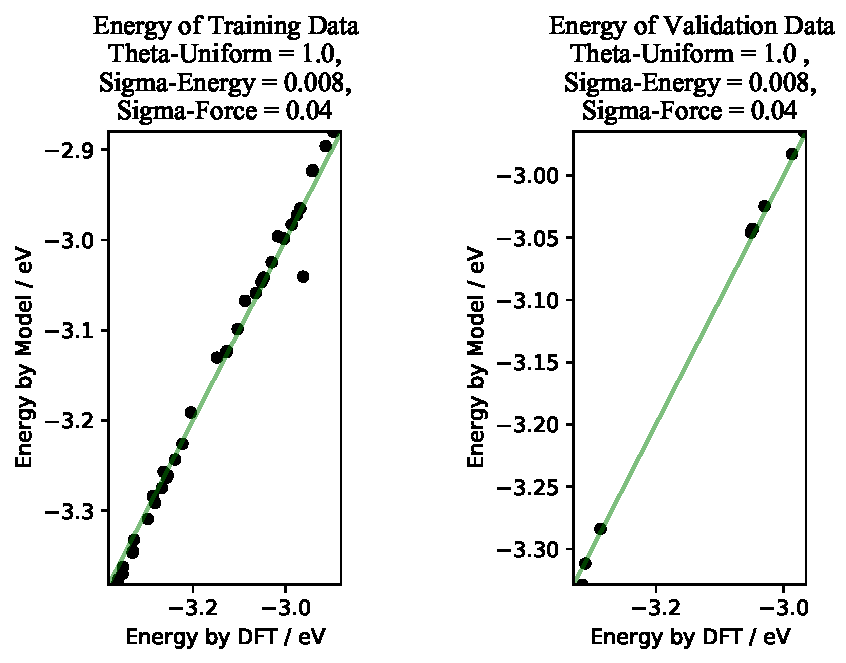
\includegraphics{../Bilder/Initial_Energies_H2.pdf}
	\caption{Energies of $H_2$ Molecule for Training Data and Validation Data before Optimisation}
	\label{epre_opt_h2}
\end{figure}

\begin{figure}
	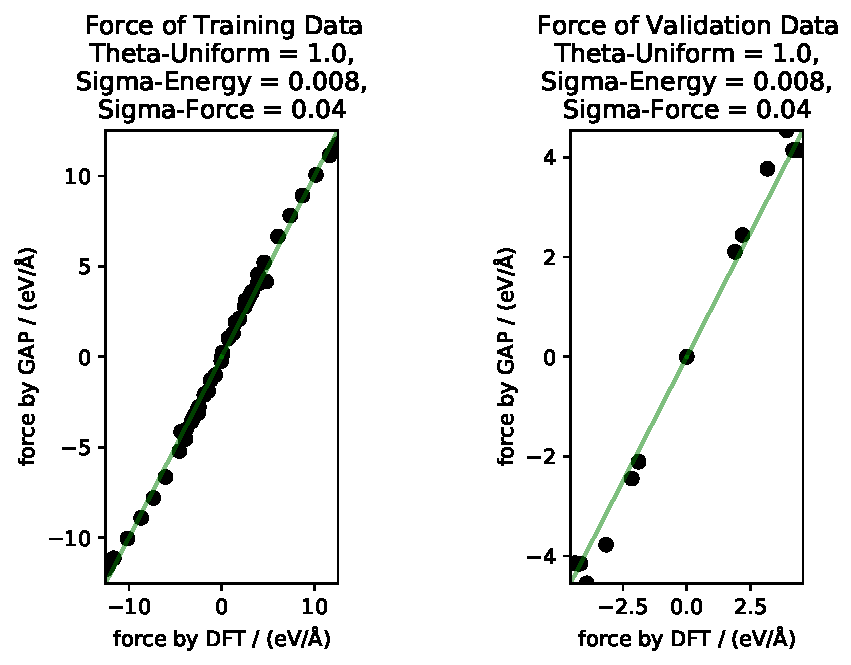
\includegraphics{../Bilder/Initial_Forces_H2.pdf}
	\caption{Forces  of $H_2$ Molecule for Training Data and Validation Data before Optimisation}
	\label{fpre_opt_h2}
\end{figure}

Fixed and variable parameters are needed in addition to the training data for creating a model, referring to \ref{subsection:4.2.4}. This set of params can be see in table \ref{tab:h2params} together with the corresponding \textit{RMSE}. 




\begin{table}
\centering
  \begin{tabular}{|l|c|c|c|c|}
    \hline
     & $\theta$ & $\sigma_E$ & $\sigma_F$  & \textit{RMSE} \\
    \hline
    Before Optimisation & 1 & 0.008 & 0.04 & 0.001276 \\
    After Optimisation &  0.325703 & 0.007972 &  0.009353 & 0.0002264 \\
    \hline
  \end{tabular}
\caption{Parameters and \texttit{RMSE} before and after Optimisation for $H_2$Molecule}
\label{tab:h2params}
\end{table}



The figures \ref{fig:epre_opt_h2} and \ref{fig:fpre_opt_h2} depict the situation before the optimisation process, hence do not match reality yet. The initial guess for the parameters $\sigma_E$ $\sigma_F$ and $\theta$  and the corresponding \texitit{RMSE} in \ref{tab:h2params} change after the model is handed to the optimisation process, explained in \ref{subsection:4.2.6}. The second line of table \ref{tab:h2params} shows the tuned  parameters together with the corresponding \textit{RMSE}.



The tuned parameters and minimised \textit{RMSE} link to the figures\ref{fig:epre_opt_h2}  and \ref{fig:fpre_opt_h2}. The energy of the training data and validation data is shown in \ref{fig:epost_opt_h2}. Respectively the force of the training data and the validation data can be seen in \ref{fig:fpost_opt_h2}.


\begin{figure}
	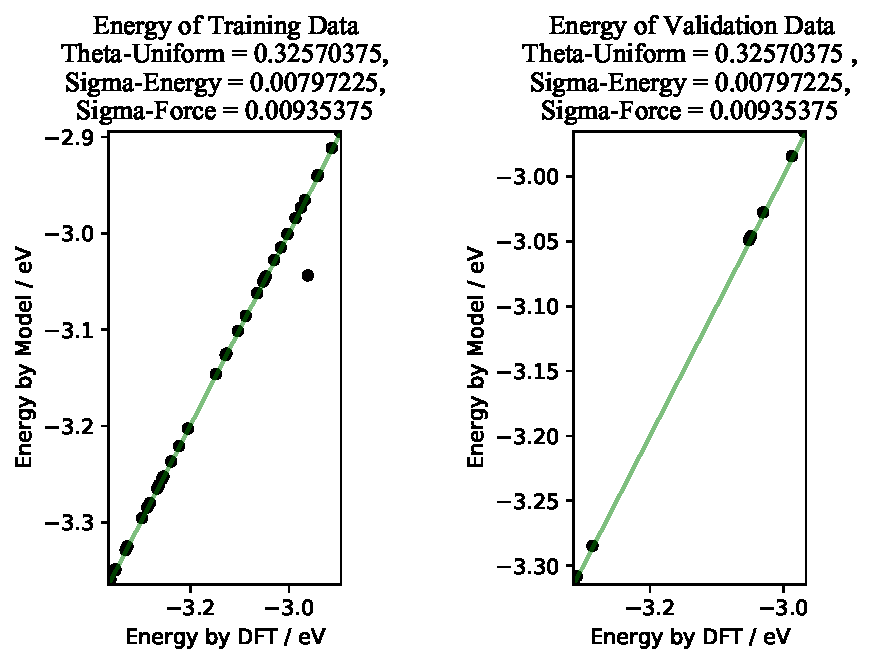
\includegraphics{../Bilder/Opt_Energies_H2.pdf}
	\caption{Energies of $H_2$ Molecule for Training Data and Validation Data after Optimisation}
	\label{epost_opt_h2}
\end{figure}

\begin{figure}
	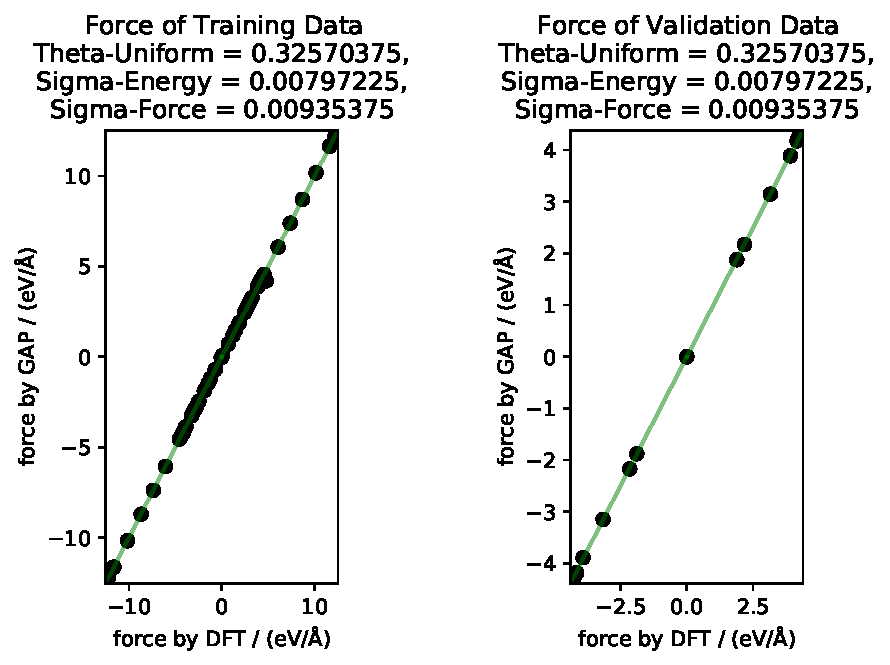
\includegraphics{../Bilder/Opt_Forces_H2.pdf}
	\caption{Forces  of $H_2$ Molecule for Training Data and Validation Data after Optimisation}
	\label{fpost_opt_h2}
\end{figure}



The optimised model leads to a smaller \textit{RMSE}, see \ref{tab:h2params} and the visual comparison of the graphs \ref{fig:epre_opt_h2} and \ref{fig:fpre_opt_h2}  to \ref{fig:epost_opt_h2}  and \ref{fig:fpost_opt_h2}  shows dots lying closer to the line for the optimised model. 


%%%%%%%%%%%%%%%%%%%%%%%%%%%%%%%%%%%%%%%%%%%%%%%%%%%%%%%%%%%%%%%%%%%%%
\subsection{Explain parameter choice, in respect to the optimisation process}
\label{subsection:5.1.2}

Performing the optimisation and tuning the parameters $\sigma_E$ $\sigma_F$ and $\theta$ leads to an almost exact mirroring of real energies and forces by the model. For the  \textit{$H_2$ Molecule} the Gradient Descent algorithm, introduced in chapter \ref{subsection:4.2.6}, terminated after 67 iterations and 137 function evaluations. 


The almost excact reproduction or real energies and forces is due to the elementariness of the examined system. The considered  \textit{$H_2$ Molecule} oscillates along the z-coordinate, hence is moving one-dimensionally. The descriptor underlying the \textit{ML-model} takes \textit{2-body distances} into account. Actual atomic configurations are transformed to a feature space.The \textit{2-body distances} descriptor feature space allows an exact representation of the  \textit{$H_2$ Molecule} oscillating in the distance between the Hydrogen Atoms. One to one mapping of the geometric atomic configuration to the feature space of the \textit{ML-Model} leads to a small \textit{RMSE} and quality classifications of the model. 





%%%%%%%%%%%%%%%%%%%%%%%%%%%%%%%%%%%%%%%%%%%%%%%%%%%%%%%%%%%%%%%%%%%%%
\subsection{Plot Dissipation Curve}
\label{subsection:5.1.3}

(Maybe, leave out for now and ask Andreas if needed)



%%%%%%%%%%%%%%%%%%%%%%%%%%%%%%%%%%%%%%%%%%%%%%%%%%%%%%%%%%%%%%%%%%%%%
\section{Outcome for Hydrogen Crystal}
\label{section:5.2}



%%%%%%%%%%%%%%%%%%%%%%%%%%%%%%%%%%%%%%%%%%%%%%%%%%%%%%%%%%%%%%%%%%%%%
\subsection{Plot real against predicted values}
\label{subsection:5.2.1}

Similarly to the \textit{$H_2$ Molecule} the \textit{Hydrogen Crystal} is examined. The system is more sophisticated due to the greater number of atoms, the $Hydrogen Crystal consists of 192 atoms compared to just two for $H_2$, but more so due to the complexity of the arrangement of the atomic constellation.  The \textit{Molecular Dynamics Simulation (MD)} starts at an unordered state. During the simulation the Hydrogen Atoms relax towards an equilibrium state.

To train and refine the model the same set of parameters is for the \textit{$H_2$ Molecule} and the \textit{Hydrogen Crystal} alike. In this chapter the goodness of the \textit{ML-Model} of the \textit{Hydrogen Crystal} is analysed. A visualisation on how the model fares to reproduce the quantum-mechanically calculated values, before the start of the optimisation process can be found in figure \ref{fig:epre_opt_hcrystal} for the energies of the training data and the validation data. The forces of the training data and for the validation data can be found in \ref{fig:fpre_opt_hcrystal}. The green diagonal line serves as target line for the predicted values. If on the line the predicted values match the real values. By looking at the figures  \ref{fig:epre_opt_hcrystal} and \ref{fig:fpre_opt_hcrystal} and checking the positions of the dots, representing the classifications of the model, one can see that the initial model does not mirror reality.


\begin{figure}
	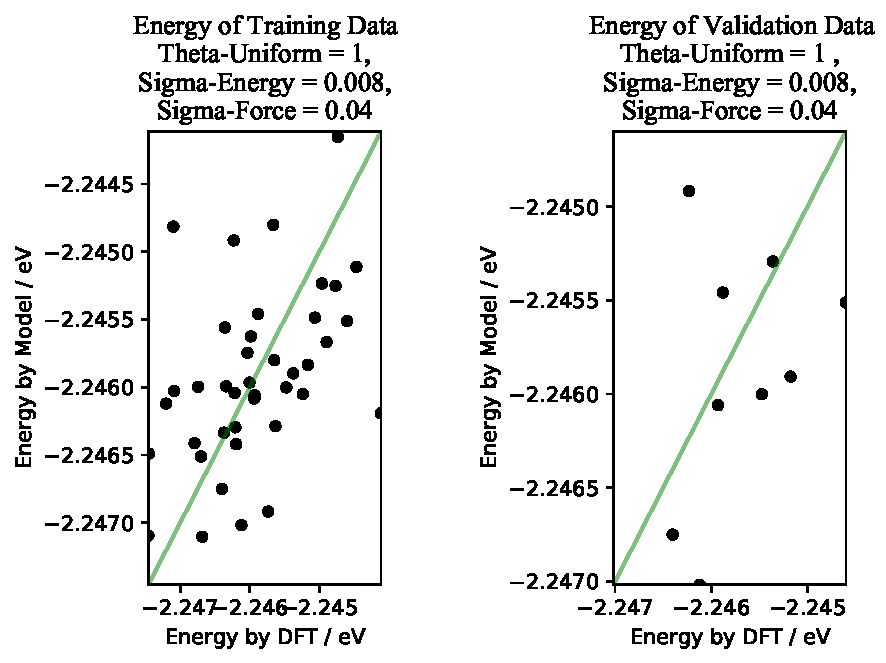
\includegraphics{../Bilder/Initial_Energies_HCrystal.pdf}
	\caption{Energies of Hydrogen Crystal for Training Data and Validation Data before Optimisation}
	\label{epre_opt_hcrystal}
\end{figure}

\begin{figure}
	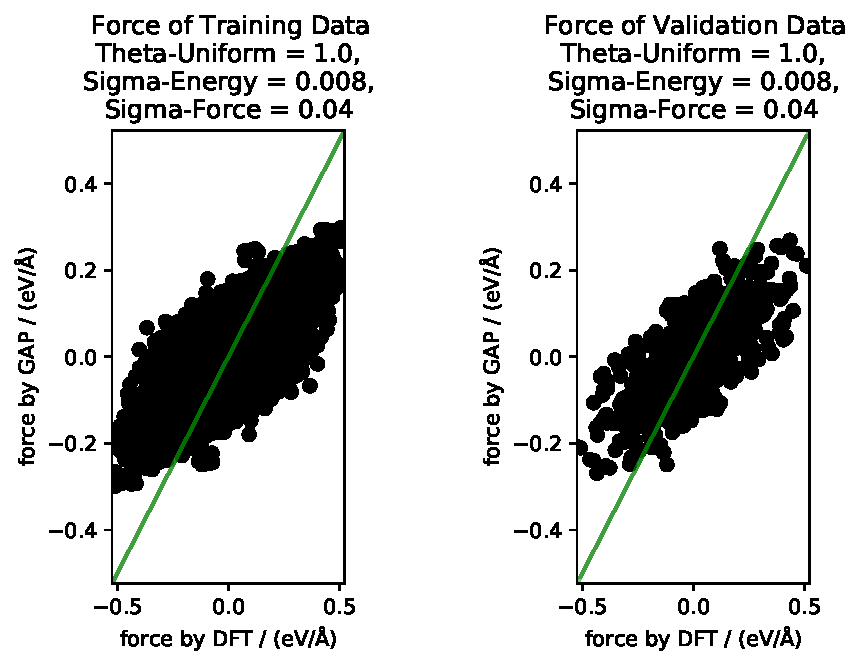
\includegraphics{../Bilder/Initial_Forces_HCrystal.pdf}
	\caption{Forces  of Hydrogen Crystal for Training Data and Validation Data before Optimisation}
	\label{fpre_opt_hcrystal}
\end{figure}




Additionally, the values of the parameters and the \textit{RMSE} can be seen in  \ref{tab:hcrystalparams}. 




\begin{table}
\centering
  \begin{tabular}{|l|c|c|c|c|}
    \hline
     & $\theta$ & $\sigma_E$ & $\sigma_F$  & \textit{RMSE} \\
    \hline
    Before Optimisation & 1 & 0.008 & 0.04 & 0.000743
 \\
    After Optimisation &  0.384155 & 0.065248 &  0.052590 & 0.000259
 \\
    \hline
  \end{tabular}
\caption{Parameters and RMSE before and after Optimisation for \textit{Hydrogen Molecule}}
\label{tab:hcrystalparams}
\end{table}


Starting out with the same set of parameters for the \textit{$H_2$ Molecule}, in   \ref{tab:h2params} and the \textit{Hydrogen Crystal}, in \ref{tab:hcrystalparams}, $\sigma_E$ $\sigma_F$ and $\theta$ change significantly after the optimisation process is run. The values for the variable parameters vary from the ones found in \ref{tab:h2params}. A visualisation of the predictions of the optimised values for the energies can be found in \ref{fig:epost_opt_hcrystal} for the training data and the validation data. Predictions on forces of the training data  and the validation data are shown in \ref{fig:fpost_opt_hcrystal}.




\begin{figure}
	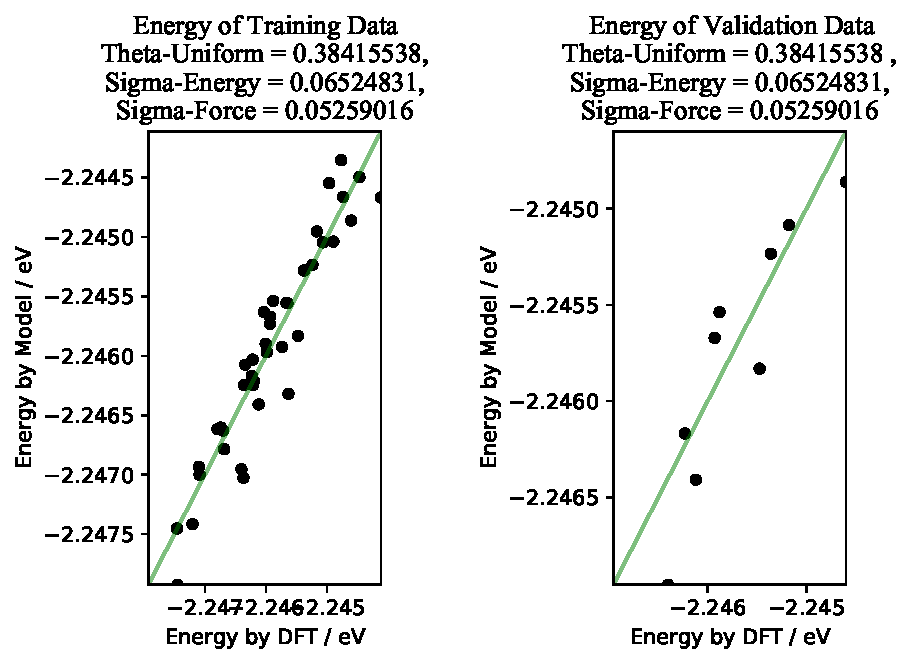
\includegraphics{../Bilder/Opt_Energies_HCrystal.pdf}
	\caption{Energies of Hydrogen Crystal for Training Data and Validation Data after Optimisation}
	\label{epost_opt_hcrystal}
\end{figure}

\begin{figure}
	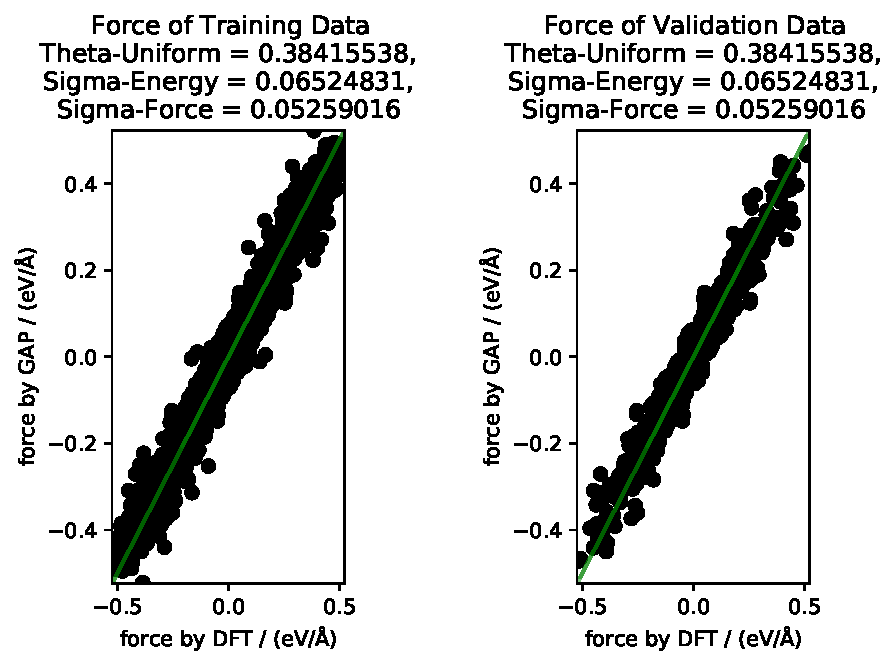
\includegraphics{../Bilder/Opt_Forces_HCrystal.pdf}
	\caption{Forces  of Hydrogen Crystal for Training Data and Validation Data after Optimisation}
	\label{fpost_opt_hcrystal}
\end{figure}

%%%%%%%%%%%%%%%%%%%%%%%%%%%%%%%%%%%%%%%%%%%%%%%%%%%%%%%%%%%%%%%%%%%%%
\subsection{Explain parameter choice, in respect to the optimisation process}
\label{subsection:5.2.2}
Two main conclusions can be drawn from the optimisation process of the model of the  \textit{Hydrogen Crystal}. First, the \texit{RMSE} error is reduced significantly throughout the optimisation process. Looking at the plots before  \ref{fig:epre_opt_hcrystal} and \ref{fig:fpre_opt_hcrystal} and after  \ref{fig:epost_opt_hcrystal} and \ref{fig:fpost_opt_hcrystal} the appliance of the optimising \textit{Gradient Descent} algorithm, one can see that the dots resembling the predicted values of energies and forces in respect to their real values have moved drastically towards the optimal green line. The reduction of the \textit{RMSE} can be seen in table \ref{tab:hcrystalparams}.  The optimisation process terminated after 46 iterations and 104 function evaluations. 

Second,  the plots in figures \ref{fig:epost_opt_hcrystal} and \ref{fig:fpost_opt_hcrystal}, together with the \textit{RMSE} in \ref{hcrystalparams} show the relatively low quality of the model compared to the \textit{$H_2 molecule$}. The predictions for the \textit{Hydrogen Crystal} feature a larger variance in respect to the corresponding real values than the predictions of the model for the  \textit{$H_2 Molecule$}. 
Looking at the predictions of the model in the figures \ref{fig:epost_opt_hcrystal} and \ref{fig:fpost_opt_hcrystal} one cannot see the that predicted and real values coincide on every occasion, but a strong trend is visible. 

The reason the model does not classify energies and forces a well as it does for the \textit{$H_2 Molecule$}  is the choice of descriptor. Building both models a {2-body-distance} descriptor has been applied. A one dimensional distance suffices the requirements of the oscillating \textit{$H_2$ Molecule} but does not so for a 192 Atom \textit{Hydrogen Crystal} relaxing to an equilibrium state. The descriptor fails to precisely map the complex 192 Atom constellation to a feature space serving as input for the \textit{ML-Model}. The loss of information by choice of a \textit{2-body-distance} descriptor determines the worse prediction performance of the model compared to the precise predictions of the model for the \textit{$H_2$ Molecule}. The interatomic interference of the larger system exceeds sphere of the simple \textit{2-body-distance} descriptor.

Fine tuning the parameters leads to the best achievable results, visualised in the plots \ref{fig:epost_opt_hcrystal} and \ref{fig:fpost_opt_hcrystal} with the values off the optimal predictions but a visible slope and a trend towards correct classification. 









